Chapter~\ref{chapter:pro_rlldb_sequence} concerns in determining the rate of \gls{RdB} sequence. Besides, designing efficient encoder and decoder for a longest \gls{RdB} sequence are also critical contributions. 

To calculate the rate and maximal asymptotic rate of \gls{RdB} sequence, first, results on the maximal length of a \gls{RdB} sequence are presented. After that, efficient algorithms to generate a longest RdB sequence and locate any sub-sequence in such sequence are also provided.

\section{Longest simple path in RdB graph}\label{sec:graph_representation}
The rate of de Bruijn sequences can be determined by understanding its longest length. Section \ref{sec:rate} provides a formal definition of rate and maximal asymptotic rate of the de Bruijn sequence. This section concerns finding the longest simple path in $G_{k,s}$, which corresponds to the longest $(k,s)$-RdB sequence.

Let $N(k,s)$ is the maximal length of a $(k,s)$-RdB sequence, and $\ell(G_{k,s})$ be the length of the longest simple path in $G_{k,s}$. Recall that a length $l$ simple path in $G_{k,s}$ is equivalent to a $(k,s)$-RdB sequence of length $l+k-1$. Therefore, $N(k,s) = \ell(G_{k,s})+k-1$. 

The de Bruijn graph $G_{k}$ is actually an Eulerian graph because each vertex has exactly two in-coming edges and two out-coming edges. This results in its longest path visiting each edge exactly once and has a length of $2^{k}$. However, $(k,s)$-RdB graph $G_{k,s}$ doesn't have the same property since the in-degree and out-degree of each vertex can be one or two. Thus, a simple path that visits all edges of the graph may not exist. 

To overcome this issue, the upper bound $\mathbb{U}(k,s)$ for the length of the longest simple path is first determined in this section. Then, $\mathcal{U}(k,s)=\mathbb{U}(k,s)+k-1$ is the upper bound for the length of longest $(k,s)$-RdB sequence. This work later proves that such bound can be achieved by proposing an efficient encoder returning a sequence of length $\mathcal{U}(k,s)$ in section \ref{subsect:encoder}. Hence, it's sufficient to conclude that the upper bound $\mathbb{U}(k,s)$ is also the length of the longest simple path. In other words, $\ell(G_{k,s})=\mathbb{U}(k,s)$, and $N(k,s)=\mathcal{U}(k,s)$

Before deriving the explicit formula of maximal length, it's necessary to analyze more meticulously the in-degree and out-degree of all vertices. Given $0\leq i,j\leq s$, define:

\begin{align*}
    V^{k-1,s}_{i,j} = \Bigl\{ \bfx: \bfx\in V^{k-1,s}, &x[1,i+1]=0^{i}1,  \\
    &x[k-1-j,k-1]=10^{j} \Bigl\}
\end{align*}

That is, $V^{k-1,s}_{i,j}$ is the set of all vertices in $G_{k,s}$ satisfying the first $i+1$ letters are $(0,0,\ldots,0,1)$ and the last $j+1$ letters are $(1,0,0,\ldots,0)$. Lemma~\ref{lem_prop_of_V_ks_ij} summaries the properties of $V^{k-1,s}_{i,j}$ the helps finding $\mathbb{U}(k,s)$.

\begin{lemma}[\textbf{Properties of $V^{k-1,s}_{i,j}$}]\label{lem_prop_of_V_ks_ij}
    {\color{white}.}
    
    % \begin{itemize}
    %     \item $\card{ V^{k-1,s}_{i,j}} = \card{ W(k-i-j-3,s)} $.
    %     \item $\sum_{0\leq i,j\leq s}\card{ V^{k-1,s}_{i,j}} = \card{ V^{k-1,s}}\ (= \card{ W(k-1,s)})$.
    %     \item The in-degree and out-degree of each vertex in $V^{k-1,s}_{i,j}$ (if $V^{k-1,s}_{i,j}\neq\emptyset$) is exactly $1$.
    %     \item The in-degree and out-degree of each vertex in $V^{k-1,s}_{i,j}$ is exactly $1$ for all $0\leq i,j\leq s-1$.
    %     \item For each vertex in $V^{k-1,s}_{s,i}\ (0\leq i\leq s-1)$, their in-degree is exactly one and their out-degree is exactly two.
    %     \item For each vertex in $V^{k-1,s}_{i,s}\ (0\leq i\leq s-1)$, their in-degree is exactly two and their out-degree is exactly one.
    % \end{itemize}
    
    \begin{enumerate}
        \item $\card{ V^{k-1,s}_{i,j}} = \card{ W(k-i-j-3,s)} $.
        \item $\sum_{0\leq i,j\leq s}\card{ V^{k-1,s}_{i,j}} = \card{ V^{k-1,s}}\ (= \card{ W(k-1,s)})$.
        \item The in-degree and out-degree of each vertex in $V^{k-1,s}_{s,S}$ (if $V^{k-1,s}_{s,s}\neq\emptyset$) is exactly $1$.
        \item The in-degree and out-degree of each vertex in $V^{k-1,s}_{i,j}$ is exactly $1$ for all $0\leq i,j\leq s-1$.
        \item For each vertex in $V^{k-1,s}_{s,i}\ (0\leq i\leq s-1)$, their in-degree is exactly one and their out-degree is exactly two.
        \item For each vertex in $V^{k-1,s}_{i,s}\ (0\leq i\leq s-1)$, their in-degree is exactly two and their out-degree is exactly one.
    \end{enumerate}
\end{lemma}
\begin{proof}
    {\color{white}.}
    
    \begin{enumerate}
        \item For each element $x\in V^{k-1,s}_{i,j}$, its subsequence, $x[i+1,k-2-j]$, can be any sequence of length $k-i-j-3$ such that more than $s$ consecutive letter $0$'s is forbidden. Hence $x[i+1,k-2-j]\in W(k-i-j-3,s)$. Reversely, given an arbitrary sequence $y\in W(k-i-j-3,s)$, the string $0^{i}1y10^{j}$ is a sequence in $V^{k-1,s}_{i,j}$. It comes to the conclusion that there is a bijection from $V^{k-1,s}_{i,j}$ to $W(k-i-j-3,s)$. In other word, $\card{ V^{k-1,s}_{i,j}} = \card{ W(k-i-j-3,s)} $.
        
        \item Since $V^{k-1,s}_{i,j}\cup V^{k-1,s}_{i^{\prime},j^{\prime}} = \emptyset$ with $(i,j)\neq(i^{\prime},j^{\prime})$, and $i,j$ cannot exceed $s$, thus, $\sum_{0\leq i,j\leq s}\card{ V^{k-1,s}_{i,j}} = \card{ V^{k-1,s}}$.
        
        \item The properties from $(3)$ to $(6)$ can be deduced directly by considering the prefix and suffix of each element in those sets.
    \end{enumerate}
\end{proof}


% For example, in case $s=1$, all vertices in $V^{k-1,1}_{1,0}$ has one edge coming in and two edges coming out. Hence, the

% All vertices in $V^{k-1,1}_{0,1}$ has two edges coming in and one edges coming out. Furthermore, among two edges coming out of each vertex $v$ in $V^{k-1,s}_{1,0}$, only one of them coming to a vertex $u$ in $V^{k-1,s}_{0,1}$. Similarly, among two edges coming to each vertex $u$ in $V^{k-1,s}_{0,1}$, only one of them coming from a vertex $v$ in $V^{k-1,s}_{1,0}$. Note that, $\card{ V^{k-1,1}_{0,1}} = \card{ V^{k-1,1}_{1,0}} = \card{ W(k-4,1)}$, therefore, there are precisely $\card{ W(k-4,1)}$ edges, each of which go from a vertex in $V^{k-1,1}_{1,0}$ to a vertex in $V^{k-1,1}_{0,1}$. If we remove all these in 

\begin{theorem}[\textbf{Longest simple path}]\label{theo:maximal_length}
    Let $C=\min{(s-1,k-s-2)}$. The length of the longest path in $G_{k,s}$, $\ell(G_{k,s})$, is equal to $\mathbb{U}(k,s)$, where:
    \begin{align}
        \mathbb{U}(k,s) = \card{ W(k,s)} - \left(\sum_{i=0}^{C}\card{ W(k-i-s-3,s)} - s\right)
    \end{align}
\end{theorem}

As mentioned above, proof of theorem \ref{theo:maximal_length} is divided into 2 parts. While the first one claims $\ell(G_{k,s})\leq\mathbb{U}(k,s)$, the second one shows that there exists a sequence can achieve the length of $\mathbb{U}(k,s)+k-1$. This section provides the proof of the first part (lemma~\ref{lem:upperbound}). Proof for the second part is available in section \ref{sec:construction}. 
    
\begin{lemma}\label{lem:upperbound}
    The longest simple path in $G_{k,s}$'s length cannot exceed $\mathbb{U}(k,s)$, that is, $\ell(k,s)\leq\mathbb{U}(k,s)$.
\end{lemma}
    The following definitions and claims are essential to prove lemma~\ref{lem:upperbound}.  
    
\begin{definition}[Balance and unbalanced vertex]
    A vertex with the quantity of in-coming edge equal to the quantity of out-coming edge is called a balanced vertex. A vertex is left-unbalanced if it has $2$ edges coming in and $1$ edges coming out. Reversely, a vertex is right-unbalanced if it has $1$ edge coming in and $2$ edges coming out.
\end{definition}

% {\color{red} Define a path to be a sequence of edges: $e_{1},e_{2},\cdots,e_{n}$ such that $\tau(e_{i})=\sigma(e_{i+1})$ where $\sigma(e_{i})$ and $\tau(e_{i})$ are initial state and terminal state of edge $e_{i}$ respectively}.

Recall that a path is defined to be a sequence of edges. A vertex $v$ is said to be (lying) in or belong to a path $\mathcal{P}$, denoted by $v\in\mathscr{P}$, if $v$ has edges in $\mathcal{P}$. It's also fair to say that $\mathcal{P}$ goes through $v$. Besides, $v$ is called the end (or the start) vertex of $\mathcal{P}$ if its last (first) edge ends (begins) at $v$.

Suppose $\mathscr{P}$ to be a longest simple path in $G_{k,s}$. In other word, $\mathscr{P}$ achieves the length $\ell(G_{k,s})$. Some observations about $\mathscr{P}$ are given in the following claims.
\begin{claim}\label{claim:equal_n_edges}
    All the vertices in $\mathscr{P}$, if not a start or end vertex, must have the number of in-edges and out-edges equal in $\mathscr{P}$.
\end{claim}
\begin{proof}
    Let $v$ be a vertex in $\mathscr{P}$, $v$ is neither start nor end vertex. Then whenever $\mathscr{P}$ comes to $v$ by an in-edge, it must go out of $v$ by an out-edge. So the claim \ref{claim:equal_n_edges} is true.
\end{proof}

% \begin{claim}\label{claim:p_not_cycle}
%     The longest simple path $\mathscr{P}$ is not a cycle.
% \end{claim}
% \begin{proof}
%     Let $\mathscr{P} = (e_{1},e_{2},\ldots,e_{n})$. Denote $\pi(e)$ and $\tau(e)$ to be initial and terminate vertices of $e$ respectively.
    
%     Assume to the contrary that $\mathscr{P}$ is a cycle. Then $\tau(e_{i})=\pi(e_{i+1})$ for all $1\leq i\leq n$, where $e_{n+1}=e_{1}$. 
    
%     \begin{enumerate}
%         \item It can be proved that there is an edge $e^{\prime}\notin \mathscr{P}$ such that either its terminal or its initial vertex $v$ is in $\mathscr{P}$.
%         \begin{itemize}
%             \item If all of vertices in $\mathscr{P}$ are balanced, since RdB graph is connected, there exists an edge (either in or out) of an vertex, for instance, $\tau(e_{i})\in\mathscr{P}$ connecting to an unbalanced vertex $u\notin\mathscr{P}$.
%             \item Otherwise, without loss of generalization, let $\tau(e_{i})$ be an left-unbalanced vertex. Since the number of in-edges and out-edges of $\tau(e_{i})$ equal (by claim~\ref{claim:equal_n_edges}), one out-edge $e^{\prime}$ of $\tau(e_{i})$ doesn't belong to $\mathscr{P}$.
%         \end{itemize}
%         \item Suppose that $e^{\prim}$ is such an edge, and $\pi(e^{\prime})=\tau(e_{i})$. Then the simple path $(e_{i+1},e_{i+2},\ldots,e_{i},e^{\prime})$ is a proper path in RdB, but longer than $\mathscr{P}$, which is a contradiction. 
%     \end{enumerate}
%     The proof is complete.
% \end{proof}

\begin{claim}\label{claim:balance_ver}
    Every balance vertex in $\mathscr{P}$ has their quantity of in-edges and out-edges in $\mathscr{P}$ equal, even if one of them is the start or end vertex.
\end{claim}
\begin{proof}
    Let $v$ be a balanced vertex and $\mathscr{P}$ goes through $v$. If $v$ is neither end nor start vertex, by claim~\ref{claim:balance_ver}, $v$ has the number of in-edges and out-edges in $\mathscr{P}$ equal. 
    
    Without loss of generality, assume that $v$ is the start vertex. This results in the number of out-edges of $v$ being equal or has $1$ edges more than its number of out-edges. If these two quantities are equal, the proof is done. Otherwise, denote $e^{\prime}$ to be one of $v$'s in-edges not belonging to $\mathscr{P}$. Then the path $\mathscr{P}_{1} = \{e^{\prime}\}\cup\mathscr{P}$ beginning at $e^{\prime}$ is a proper simple path RdB graph, but longer than $\mathscr{P}$, which contradicts to the assumption about the longest property of $\mathscr{P}$.
\end{proof}
\begin{claim}\label{claim:shortes_right-left}
    Let $u=0^{s}1x1_{t}0^{j}$ be a right-unbalanced vertex. Then the shortest path going from $u$ to an arbitrary left-unbalanced vertex lengthen $s-j$.
\end{claim}
\begin{proof}
    A left-unbalanced vertex is represented by a sequence whose suffix of length $s$ is filled by $0$. Hence, a path from $u$ to a left-unbalanced vertex must contain at least $s-j$ edges labeled $0$. In fact, a path of length $s-j$ connecting $u$ to a left-unbalanced vertex exists, which is the path of all $0$ labeled edges. This path comes from $u$ to $0^{s-j}1x1_{t}0^{s}$.
\end{proof}
% \begin{proof}
%     Let $v$ be a vertex in $\ell(G_{k,s})$. We just need to consider if $v$ is start or end vertex, the other cases have already been proved by claim \ref{claim:equal_n_edges}.
    
%     Assume that $v$ is the start vertex and suppose to the contrary 
% \end{proof}

\begin{proof}[Proof for lemma~\ref{lem:upperbound}]
    Define $1x1_{t}$ to be a sequence of length $t$ such that start and end letters are both $1$. Let $$\mathscr{L}=\bigcup_{j=0}^{C}\left\{\bfu:\bfu=0^{j}1x1_{t}0^{s},s+t+j=k-1\right\}$$ be the set of all left-unbalanced vertices
    
    Let $\bfv=0^{j}1x1_{t}0^{s}$ be an arbitrary vertex in $\mathscr{L}$ such that $\bfv$ isn't the end-vertex of path $\mathscr{P}$. 
    
    \begin{enumerate}
        \item It can be proved that there is a path $\mathcal{P}_{v}$ of length $s-j$ satisfying all of its edges not lying in $\mathscr{P}$ and its end-vertex is $\bfv$.
            The path $\mathcal{P}_{v}$ is constructed backwardly as follows:
            
            Starts with $\mathcal{P}_{v}=\emptyset$. As $\bfv$ has $2$ in-edges and $1$ out-edges, there's at least $1$ in-edge $e_{v}$ of $\bfv$ not lying in $\mathscr{P}$. Of course, $e_{v}$'s label is $0$. Adds $e_{v}$ to $\mathscr{P}_{v}$. Let $a_{1}0^{j}1x1_{t}0^{s-1}= \pi(e_{v})$ be the initial state of $e_{v}$. If $\pi(e_{v})$ is a balance vertex, then by the claim \ref{claim:balance_ver}, there also must be at least $1$ in-edge of $\pi(e_{v})$ not lying in $\mathscr{P}$. Continue adding this edge to the head of $\mathcal{P}_{v}$. Denote $a_{2}a_{1}0^{j}1x10^{s-2}$ to be the initial state of this edge. Now, $\mathcal{P}_{v}$ can be represented as below:
            
            \[\mathcal{P}_{v}=\left[\left(a_{2}a_{1}0^{j}1x1_{t}0^{s-2},a_{1}0^{j}1x1_{t}0^{s-1}\right), \left(a_{1}0^{j}1x1_{t}0^{s-1},0^{j}1x1_{t}0^{s}\right)\right]\]
            
            Assume inductively that:
            
            \begin{align*}
                \mathcal{P}_{v}= \Bigl[&\left(a_{l}\cdots a_{2}a_{1}0^{j}1x1_{t}0^{s-l},a_{l-1}\cdots a_{1}0^{j}1x1_{t}0^{s-(l-1)}\right),\cdots,\\
                &\left(a_{2}a_{1}0^{j}1x1_{t}0^{s-2}, a_{1}0^{j-1}1x1_{t}0^{s-1}\right),\\
                &\left(a_{1}0^{j-1}1x1_{t}0^{s-1},0^{j}1x1_{t}0^{s}\right)\Bigl]   
            \end{align*}
            with $l\leq s-j$.
            
            If $l=s-j$, the proof is done. Otherwise, it's obvious that $$a_{l}\cdots a_{2}a_{1}0^{j}1x1_{t}0^{s-l}$$ is balance, hence, by claim \ref{claim:balance_ver}, it also has at least $1$ in-edge not lying in $\mathscr{P}$, and one can continue adding such edge to the head of $\mathcal{P}_{v}$.
            
        \item It can be shown that for each $u,v\in\mathscr{L}$ such that neither $u$ nor $v$ is the end vertex of the last edge of $\mathscr{P}$, paths $\mathcal{P}_{u}$ and $\mathcal{P}_{v}$ are edge-disjoint.
    
            Represent $\mathcal{P}_{u} = [e_{u,1},e_{u,2},\cdots,e_{u,i}]$, $\mathcal{P}_{v}=[e_{v,1},e_{v,2},\cdots,e_{v,j}]$. Assume to the contrary that $\exists t\leq i,l\leq j$ satisfying $e_{u,t}=e_{v,l}$. Without loss of generalization, we suppose that $i-t\leq j-l$. As all edges in $\mathcal{P}_{u}$ and $\mathcal{P}_{v}$ are labeled $0$, we must have $e_{u,t+1}=e_{v,l+1},\cdots,e_{u,i}=e_{v,l+(i-t)}$. 
            
            If $l+i-t=j$, we have $\mathcal{P}_{u}$ and $\mathcal{P}_{v}$ have the same last edge but different terminal states, which is impossible. Otherwise, the path $e_{v,l+i-t+1},\cdots,e_{v,j}$ is the path connecting $u$ to $v$. But the length of this path is smaller than $s$, which is also absurd.
    \end{enumerate}
    % $(1)$ It can be proved that there is a path $\mathcal{P}_{v}$ of length $s-j$ satisfying all of its edges not lying in $\mathscr{P}$ and its end-vertex is $\bfv$.
    
    % The path $\mathcal{P}_{v}$ is constructed backwardly as follow:
    
    % Starts with $\mathcal{P}_{v}=\emptyset$. As $\bfv$ has $2$ in-edges and $1$ out-edges, there's at least $1$ in-edge $e_{v}$ of $\bfv$ not lying in $\mathscr{P}$. Of course, $e_{v}$'s label is $0$. Adds $e_{v}$ to $\mathscr{P}_{v}$. Let $a_{1}0^{j}1x1_{t}0^{s-1}= \pi(e_{v})$ be the initial state of $e_{v}$. If $\pi(e_{v})$ is a balance vertex, then by the claim \ref{claim:balance_ver}, there also must be at least $1$ in-edge of $\pi(e_{v})$ not lying in $\mathscr{P}$. Continue adding this edge to the head of $\mathcal{P}_{v}$. Denote $a_{2}a_{1}0^{j}1x10^{s-2}$ to be the initial state of this edge. Now, $\mathcal{P}_{v}$ can be represented as below:
    
    % $\mathcal{P}_{v}=[\left(a_{2}a_{1}0^{j}1x1_{t}0^{s-2},a_{1}0^{j}1x1_{t}0^{s-1}\right), \left(a_{1}0^{j}1x1_{t}0^{s-1},0^{j}1x1_{t}0^{s}\right)]$
    
    % Assume inductively that:
    
    % \begin{align*}
    %     \mathcal{P}_{v}= \Bigl[&\left(a_{l}\cdots a_{2}a_{1}0^{j}1x1_{t}0^{s-l},a_{l-1}\cdots a_{1}0^{j}1x1_{t}0^{s-(l-1)}\right),\cdots,\\
    %     &\left(a_{2}a_{1}0^{j}1x1_{t}0^{s-2}, a_{1}0^{j-1}1x1_{t}0^{s-1}\right),\\
    %     &\left(a_{1}0^{j-1}1x1_{t}0^{s-1},0^{j}1x1_{t}0^{s}\right)\Bigl]   
    % \end{align*}
    % with $l\leq s-j$.
    
    % If $l=s-j$, the proof is done. Otherwise, it's obvious that $a_{l}\cdots a_{2}a_{1}0^{j}1x1_{t}0^{s-l}$ is balance, hence, by claim \ref{claim:balance_ver}, it also has at least $1$ in-edge not lying in $\mathscr{P}$, and one can continue adding such edge to the head of $\mathcal{P}_{v}$.
    
    % $(2)$ It can be shown that for each $u,v\in\mathscr{L}$ such that neither $u$ nor $v$ is the end vertex of the last edge of $\mathscr{P}$, paths $\mathcal{P}_{u}$ and $\mathcal{P}_{v}$ are edge-disjoint.
    
    % Represent $\mathcal{P}_{u} = [e_{u,1},e_{u,2},\cdots,e_{u,i}]$, $\mathcal{P}_{v}=[e_{v,1},e_{v,2},\cdots,e_{v,j}]$. Assume to the contrary that $\exists t\leq i,l\leq j$ satisfying $e_{u,t}=e_{v,l}$. Without loss of generalization, we suppose that $i-t\leq j-l$. As all edges in $\mathcal{P}_{u}$ and $\mathcal{P}_{v}$ are labeled $0$, we must have $e_{u,t+1}=e_{v,l+1},\cdots,e_{u,i}=e_{v,l+(i-t)}$. 
    
    % If $l+i-t=j$, we have $\mathcal{P}_{u}$ and $\mathcal{P}_{v}$ have the same last edge but different terminal states, which is impossible. Otherwise, the path $e_{v,l+i-t+1},\cdots,e_{v,j}$ is the path connecting $u$ to $v$. But the length of this path is smaller than $s$, which is also absurd.
    
    Summary, for each vertex in $\mathscr{L}$ such that $v$ isn't the end-vertex of the last edge in path $\mathscr{P}$, there is a path $\mathcal{P}_{v}$ of length $s-j$ satisfying all of its edges not lying in $\mathscr{P}$ and takes $v$ to be its end-vertex. Moreover, all these such paths are edge-disjoint, and there can be only $1$ end-vertex of the last edge in path $\ell(G_{k,s})$, the total edges of all such path $\mathcal{P}_{u}$ is:
    \begin{align*}
        \sum_{i=0,i\neq j}^{C} &(s-i)\lvert W(k-s-i-3,s) \rvert \\
        + &(s-j)(\lvert W(k-s-j-3,s)\rvert-1)\\
        = \sum_{i=0}^{C} &(s-i)\lvert W(k-s-i-3,s) \rvert - (s-j) \\
        \geq \sum_{i=0}^{C} &(s-i)\lvert W(k-s-i-3,s) \rvert -s  
    \end{align*}
    This means at least $\sum_{i=0}^{C} (s-i)\lvert W(k-s-i-3,s) \rvert -s$ edges not lying in $\mathscr{P}$. As the number of edges in $(k,s)$-RdB is $\lvert W(k,s)\rvert$, the length of the longest path $\mathscr{P}$ can not exceed : 
    \[\lvert W(k,s)\rvert - (\sum_{i=0}^{C} (s-i)\lvert W(k-s-i-3,s) \rvert- s)\]
    This concludes our lemma.
\end{proof}

Define $\mathcal{U}(k,s) = \mathbb{U}(k,s)+(k-1)$, then $\mathcal{U}(k,s)$ is length of the longest $(k,s)$-RdB sequence.

\section{Rate and maximal asymptotic rate of \texorpdfstring{$(k,s)$}{(k,s)}-RdB sequence}\label{sec:rate}
For every $(k,s)$-RdB sequence, their rate is defined as follows:
\begin{definition}[Rate]
    Denote $R(\bfx_{k,s})$ to be the rate of a $(k,s)$-RdB sequence $\bfx_{k,s}$, then:
    \begin{align}
        R(\bfx_{k,s}) = \dfrac{\log\left(\card{\bfx_{k,s}}\right)}{k}
    \end{align}
    where the base of logarithm function is $\left\lvert\Sigma\right\rvert=2$.
\end{definition}

The rates of sequences are the proportion of the data-stream that is useful (non-redundant), tell how much useful information is transmitted. The sequence's rate actually originates from information rate. Recall that, in definition~\ref{def:information_rate}, the rate $R_{C}$ of a code $C$ consisting of length $n$ $q$-ary sequences is $R_{C}=\dfrac{\log_{q}\left(\card{C}\right)}{n}$. If a $(k,s)$-RdB sequence $x_{k,s}$ is considered to be a code $C_{k,s}$, each of its size $k$ windows is treated as a codeword. The size of $C_{k,s}$ is exactly the length of $x_{k,s}$ minus $k$, but the offset $k$ can be omitted under log calculation. Hence: $$R_{C_{k,s}}= \dfrac{\log_{q}\left(\card{C_{k,s}}\right)}{n} = \dfrac{\log(\card{\bfx_{k,s}})}{k} = R(x_{k,s})$$. That is to say, $R(\bfx_{k,s})$ is eventually a kind of information rate.

Note that, a high rate is usually preferred. Accordingly, with each given pair $(k,s)$, the maximal rate of all $(k,s)$-RdB sequence is defined.
\begin{definition}[Maximal rate]
    Given $k$ and $s$, the maximal rate $R_{k,s}$ of all $(k,s)$-RdB sequences is:
    \begin{align}
        R_{k,s} = \dfrac{\log(N(k,s))}{k}
    \end{align}
\end{definition}

% For the rate $R_{k,s}$, if one cares about the very large $k$, it is when the maximal asymptotic rate of sequence comes to play.

The maximal asymptotic rate is concerned in case $k$ appears to be very large.
\begin{definition}[Maximal asymptotic rate]
    Denote $R_{s}$ to be the maximal asymptotic rate of $(k,s)$-RdB sequences, then:
    \begin{align}
        R_{s} = \lim_{k\to\infty}\dfrac{\log(N(k,s))}{k}
    \end{align}
\end{definition}

Having the explicit formula of $N(k,s)$ determined makes it easier to calculate the maximal asymptotic rate of the $(k,s)$-RdB sequence. The following equation is a direct consequence of theorem~\ref{theo:maximal_length}:
\begin{align}
    N(k,s) = \card{ W(k,s)} - \left(\sum_{i=0}^{C}\card{ W(k-i-s-3,s)} - s\right) + k - 1\label{eq:N_k_s}
\end{align}


Theorem \ref{theo:rate_1} below shows that the rate of $(k,1)$-RdB sequence is better than the rate of Hybrid de Bruijn sequence. Therefore, it's able to use $(k,1)$-RdB sequence for the system in \cite{zhang2021timing} instead to increase rate, speed of encoding and decoding for the transmitted signals.

\begin{theorem}\label{theo:rate_1}
    \begin{align}
        R_{1} = 0.6942
    \end{align}
\end{theorem}
\begin{proof}
    Substitute $s=1$ into expression~\ref{eq:N_k_s} gives $N(k,1) = \card{W(k,1)} - \card{W(k-4,1)}$, and recall that $\{\card{W(k,1)}\}$ is a Fibonacci sequence with: 
    \[\card{W(k,1)} = \dfrac{\phi^{k+2}+\varphi^{k+2}}{\sqrt{5}}\].
    where $\phi = \dfrac{1+\sqrt{5}}{2}$ and $\varphi = \dfrac{1-\sqrt{5}}{2}$. Here, observe that $\phi\varphi=-1$, so $\phi^{2}\varphi^{2}=1$, consequently, it's able to write:
    \begin{align*}
        \left\{\begin{matrix}
            \phi^{-2} = \varphi^{2} \\
            \varphi^{-2} = \phi^{2}
        \end{matrix}\right.
    \end{align*}
    As a result: 
    \begin{align*}
        \card{W(k,1)} - \card{W(k-4,1)} &= \dfrac{\phi^{k+2}+\varphi^{k+2}}{\sqrt{5}} - \dfrac{\phi^{k-2}+\varphi^{k-2}}{\sqrt{5}}\\
        &= \dfrac{\phi^{k+2}+\varphi^{k+2}-\phi^{k}\varphi^{2}-\varphi^{k}\phi^{2}}{\sqrt{5}}\\
        &= \left(\phi^{k}+\varphi^{k}\right).\dfrac{\phi^{2}-\varphi^{2}}{\sqrt{5}}
    \end{align*}
    And hence:
    \begin{align*}
        R_{1} &= \lim_{k\to\infty}\dfrac{\log(N(k,1))}{k} \\
        &= \lim_{k\to\infty}\dfrac{ \log\left( \left(\phi^{k}+\varphi^{k}\right).\dfrac{\phi^{2}-\varphi^{2}}{\sqrt{5}}+k \right) }{k} \\
        &= \log(\phi) \approx 0.6942
    \end{align*}
\end{proof}

The following theorem is the generalization of theorem \ref{theo:rate_1}.
\begin{theorem}[Maximal asymptotic rate of RdB sequence]\label{theo:rate_s}
    Let $k$ be a positive integer. Then:
    \begin{align}
        R_{s} = \log(\lvert\omega\rvert)
    \end{align}
    where $\omega$ is the root of equation: %\inlineequation[eq:inline]{x^{s+1}-x^{s}-\ldots-x-1 = 0}
    \begin{equation}
        x^{s+1}-x^{s}-\ldots-x-1 = 0\label{eq:char_eq}
    \end{equation}
    such that $\lvert\omega\rvert$ is largest.
\end{theorem}
\begin{proof}
    
    The root $\omega$ is actually a Pisot number. More particularly, $\omega$ is the only positive roots of~\ref{eq:char_eq} lying in the interval $(1,2)$, the other roots are in the open disk $\left\{z\in\mathbb{C},\card{z}<1\right\}$. Also, note that $x^{s+1}-x^{s}-\ldots-x-1=0$ is the characteristic equation of $W(k,s)$. Therefore, with $k$ big enough, $\card{W(k,s)}$ can be estimated as follows: \[\card{W(k,s)} \approx a.\lvert\omega\rvert^{k}\] whereas $a$ is a positive constant. Thus, from expression~\ref{eq:N_k_s}:
    \begin{align*}
        N(k,s) &= \card{ W(k,s)} - \left(\sum_{i=0}^{C}\card{ W(k-i-s-3,s)} - s\right) + k - 1 \\
        &\approx \sum_{t=k-s}^{k}(k-t+1)a\lvert\omega\rvert^{t-2} + s + k - 1\\
        &= \lvert\omega\rvert^{k-s-2}\left( \sum_{t=k-s}^{k}a(k-t+1)\lvert\omega\rvert^{t-k+s} + \dfrac{s+k-1}{\lvert\omega\rvert^{k-s-2}}\right)\\
        &= \lvert\omega\rvert^{k-s-2}\left( \sum_{i=0}^{s}a(i+1)\lvert\omega\rvert^{s-1} + \dfrac{s+k-1}{\lvert\omega\rvert^{k-s-2}}\right) 
    \end{align*}

    This results in:
    \begin{align*}
        R_{k} &= \lim_{k\to\infty}\dfrac{\log\left( \lvert\omega\rvert^{k-s-2}\left(\sum_{i=0}^{s}a(i+1)\lvert\omega\rvert^{s-1}+\dfrac{s+k-1}{\lvert\omega\rvert^{k-s-2}}\right)\right)}{k} \\
        &= \lim_{k\to\infty}\dfrac{(k-s-2)\log(\lvert\omega\rvert)}{k} + \lim_{k\to\infty}\dfrac{\log\left(\sum_{i=0}^{s}a(i+1)\lvert\omega\rvert^{s-i}+\dfrac{s+k-1}{\lvert\omega\rvert^{k-s-2}}\right)}{k}\\
        &= \log(\lvert\omega\rvert)
    \end{align*}
    
\end{proof}
% \begin{figure*}[!ht]
%     \centering
%       \begin{subfigure}{0.9\linewidth}
%         \centering
%         \includegraphics[scale=0.23]{fig/Legend.png}
%         \label{fig:neg_size}
%         \end{subfigure}
%         %\quad
%       \begin{subfigure}{0.4\linewidth}
%         \centering
%         \includegraphics[scale=0.35]{fig/train_percent_Hit@1.pdf}
%         \caption{Hit@1}
%         \label{fig:sub_hit1}
%         \end{subfigure}
%         %\quad
%       \begin{subfigure}{0.4\linewidth}
%         \centering
%         \includegraphics[scale=0.35]{fig/train_percent_Hit@10.pdf}
%         \caption{Hit@10}
%         \label{fig:sub_hit10}
%         \end{subfigure}
%         %\quad
%     \begin{subfigure}{0.4\linewidth}
%         \centering
%         \includegraphics[scale=0.35]{fig/train_percent_MRR.pdf}
%         \caption{MRR}
%         \label{fig:sub_mrr}
%         \end{subfigure}
%     \caption{Saving of labelling effort for entity alignment on D-W-V1 test set}
%     \label{fig:supervision_percent}
%  \end{figure*}

\section{Construction of RdB sequence}\label{sec:construction}
% {\color{red} Need paraphrase to avoid self-plagiarism\color{blue}

This section presents a construction of a $(k,s)$-RdB sequence $\bfc_{k,s}$. Furthermore, given a substring of length $k$ of the sequence $\bfc_{k,s}$, a fast decoding algorithm to determine the location of the given substring is provided. The complexity of the decoding algorithm is sub-linear with respect to the length of $\bfc_{k,s}$. There are some classical de Bruijn sequences with sub-linear decoding algorithm \cite{mitchell1996method,tuliani2001bruijn,kociumaka2016efficient}. This work uses the minimal de Bruijn sequence, constructed in \cite{kociumaka2016efficient,fredricksen1978necklaces}, and some special properties of Lyndon words to construct a $(k,s)$-RdB.
% }

\begin{definition}[\textbf{Lyndon words}]
    A sequence $w$ is a Lyndon word if and only if it's strictly smaller than all of its rotation.
\end{definition}
For more intelligible, several Lyndon words and non-Lyndon words are provided in example~\ref{exp:Lyndon}.
\begin{example}[Lyndon words]\label{exp:Lyndon}
    The word $00101$ is a Lyndon word, since it is smaller than all of its rotation: $01010$, $10100$, $01001$, $10010$. The word $01100$ is not a Lyndon word, since one of its rotations, $00011$, is smaller than it. The word $011011$ is also not a Lyndon word, as its cyclic rotation by $3$ letters is equal to it. 
\end{example}

\subsection{Encoder for a\texorpdfstring{$(k,s)$}{(k,s)}-RdB sequence} \label{subsect:encoder}
In 1978, Fredricksen and Maiorana~\cite{fredricksen1978necklaces} proposed the \gls{fkm} algorithm to efficiently construct the lexicographically minimal de Bruijn sequence, which is later called granddaddy sequence by Knuth~\cite{knuth2013art}. The algorithm was based on their finding of the connection between de Bruijn sequence and Lyndon words.

\begin{lemma}[\cite{fredricksen1978necklaces}]\label{lem:FKM}
    The lexicographically minimal de Bruijn sequence of order $k$ ($k$-MdB) is the concatenation of all Lyndon words whose length is a divisor of $k$ in the lexicographically order.
\end{lemma}

For example, the $6$-MdB sequence is decomposed into Lyndon words as follows:
\begin{example}[Decomposition of $6$-MdB sequence]
    Recall that $6$-MdB sequence is already given in example~\ref{exp:granddaddy}, which is:
    \[0000001000011000101000111001001011001101001111010101110110111111\]
    As stated in lemma~\ref{lem:FKM}, it can be decomposed in lexicographically order into Lyndon words listed follows:
    \begin{align*}
        &0\\
        &000001\\
        &000011\\
        &000101\\
        &000111\\
        &001\\
        &001011\\
        &001101\\
        &001111\\
        &01\\
        &010111\\
        &011\\
        &011111\\
        &1
    \end{align*}
\end{example}


This thesis observes that it is able to append a prefix to a suffix of $k$-MdB to obtain a $(k,s)$-RdB sequence, i.e., in the cycle representing $k$-MdB, there are arcs representing $(k,s)$-RdB sequences. To illustrate this idea, figure~\ref{fig:substring_of_circle} gives an example for $k=6$ and $s=2$, where the blue arc and the red arc indicate the prefix and the suffix respectively. Any substring of the concatenation of the prefix and suffix is a $(6,2)$-RdB sequence.

\begin{figure}[htbp]
    \centering
    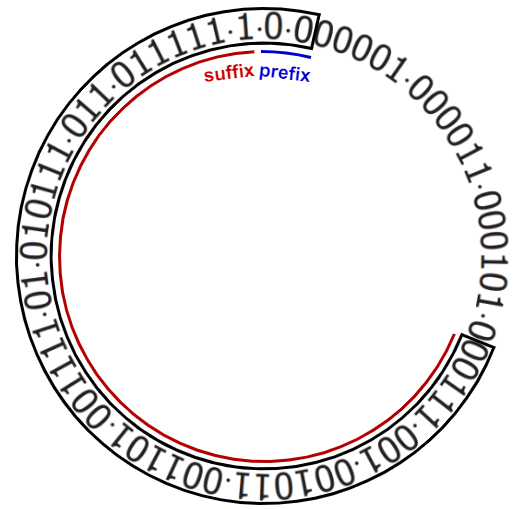
\includegraphics[scale=0.5]{fig/construction/subtring of cyclic.png}
    \caption{Example for $k=6,\ s=2$. In the circle of $6$-MdB, an arbitrary substring of the concatenation of suffix and prefix in the picture is a $(6,2)$-RdB sequence.}
    \label{fig:substring_of_circle}
\end{figure}

% \begin{figure}
%     \centering
%     \input{fig/construction/construction}
%     \caption{Caption}
%     \label{fig:my_label}
% \end{figure}

More precisely, the construction is described as follow:
\begin{construction}\label{constr:encoder}
    Let $\bfx=(x_{1},\ldots,x_{n})$ be the $k$-MdB constructed from Lemma~\ref{lem:FKM} and $u_{k,s}= 0^{s+1}1^{k-s-1}$ be a Lyndon word of length $k$ satisfying the first $s+1$ letters are all $0$'s and the last $k-s-1$ letters are all $1$'s. By the intrinsic property of de Bruijn sequences, there exists only one index $i$ such that $\bfu_{k,s}=\bfx[i,i+k-1]=(x_{i},\ldots,x_{i+k-1})$. Denote the word $\bfc_{k,s} = (x_{i+1},\ldots,x_{n},0,0,\ldots,0)$, obtained by adding $s$ letters $0$ to the end of the suffix of $\bfx$, from index $i+1$ to the end. Theorem \ref{theo:validity} below claims that $\bfc_{k,s}$ is a $(k,s)$-RdB sequence. 
\end{construction}

This thesis later proves that $\bfc_{k,s}$ is even the longest $(k,s)$-RdB sequence. 

Denote \L$_{n}$ to be the set of all Lyndon words of length $n$, and $\text{\L}^{(n)}=\cup_{d\card n}\text{\L}_{d}$ to be the set of all Lyndon words whose lengths are divisors of n. The formal encoder to construct a $(k,s)$-RdB sequence is given in algorithm~\ref{alg:encoder}.

\begin{algorithm}
\DontPrintSemicolon
    \SetKwInOut{KwIn}{Input}
    \SetKwInOut{KwOut}{Output}
    \KwIn{$k$, and descending ordered set \L$^{(n)}$. }
    \KwOut{ $(k,s)$-RLL dBs}
    \BlankLine
        % Find the set of Lyndon words  $S=\left\{\lambda_{i}:\ \lambda_{i}\in\mathsf{L}^{(k)}\right\}$
    
    $\mathbf{w}\gets$emptystring\;
    \For{$\lambda \in$\L$^{(n)}$}{
        $\mathbf{w}.prepend(\lambda)$\;
        \If{$\lambda== 0^{s+1}1^{k-s-1}$}{
            \tcc{remove the first letter of $w$, which is 0, and add $s$ letters $0$ to the end}
            $\mathbf{w} = \mathbf{w}[2,\ell]0^{s}$\;
            \textbf{break}\;
        }
    }
    \KwRet{$\mathbf{w}$}
    \caption{Encode (k,s)-RLL dBs}
    \label{alg:encoder}
\end{algorithm}

The set $\text{\L}^{(n)}$ in lexicographically order can be generated in constant amortized time by applying \gls{fkm} algorithm (analyzed in~\cite{ruskey1992generating}), or by another algorithm developed by Duval in~\cite{duval1988generation}. In algorithm~\ref{alg:encoder}, the most consuming time step is to produce the set $\text{\L}^{(n)}$, and hence, its complexity is the complexity of the algorithm used to bring out $\text{\L}^{(n)}$.
% {\color{red} Runtime of Encoder, critical runtime is at FKM ...}

Here presents an example for $k=6$ and $s=2$. 
\begin{example}[Construction of $(6,2)$-RdB sequence]
    The suffix: $$00111\ 001011\ 001101\ 001111\ 01\ 010111\ 011\ 011111\ 1$$ is taken from the granddaddy of order $6$ given above. Adding $2$ letter $0$ to the end of it obtains:
    \[
        00111\ 00\ 001011\ 001101\ 001111\ 01\ 010111\ 011\ 011111\ 1\ 00
    \]
    which is indeed a $(6,2)$-RdB sequence.
\end{example}
Now, theorem \ref{theo:validity} proves that the Construction~\ref{constr:encoder} always return a $(k,s)$-RdB sequence.

\begin{theorem}\label{theo:validity}
    The sequence $\bfc_{k,s}$ obtained from Construction~\ref{constr:encoder} is a $(k,s)$-RdB sequence.
\end{theorem}
\begin{proof}
    First, it's necessary to show that each substring of length $k$ appears at most once in $\bfc_{k,s}$. Note that the granddaddy sequence $\bfx$ obtained from Lemma~\ref{lem:FKM} is a cyclic de Bruijn sequence, and $\bfc_{k,s}$ is actually a substring of $\bfx$. Hence, $\bfc_{k,s}$ just contains each substring of size $k$ at most once.
    
    Now, claiming that $\bfc_{k,s}$ doesn't contain any patterns $0^{s+1}$ will complete the theorem. This can be proved by considering the property of Lyndon words. It's obvious to see that $\bfu_{k,s}=0^{s+1}1^{k-s-1}$ is the largest Lyndon word containing $s+1$ consecutive symbols $0$. Hence, every Lyndon words decomposed from $\bfc_{k,s}$ doesn't take $0^{s+1}$ as a substring. Moreover, the last symbol of all Lyndon words but $0$ is $1$. Therefore, $0^{s+1}$ will not appear in the combination of Lyndon words larger than $\bfu_{k,s}$. Adding $0^{s}1^{k-s-1}$ to the beginning and $s$ letters $0$ to the end of this combination resulting in $\bfc_{k,s}$ won't change this property. So, it's able to conclude that $\bfc_{k,s}$ is indeed a $(k,s)$-RdB sequence.
\end{proof}

\subsection{Decoder for a \texorpdfstring{$(k,s)$}{(k,s)}-RdB sequence}
In~\cite{zhang2021timing}, the Hybrid de Bruijn sequence of order $k$ after being received needs to be decoded for correcting errors. More particularly, it's necessary to indicating the exact location of an arbitrary sequence of length $k$ in the Hybrid de Bruijn sequence. To do that, they proposed to use look-up table, which is {\color{blue} is an exponential complex method}.

Similarly, it's essential for this work to decode $\bfc_{k,s}$. In 2016, Kociumaka, Radoszewski, and Rytter presented the first sub-linear decoding algorithm $\cD_{KRR}$ for the minimal de Bruijn sequences. And since $\bfc_{k,s}$ is a substring of a minimal de Bruijn sequence, it's able to modify $\cD_{KRR}$ to decode $\bfc_{k,s}$ in sub-linear time. 

Let $i=\cD_{KRR}(\bfu_{k,s})$ be the position of the word $\bfu_{k,s}$ in the granddaddy sequence of order $k$ $\bfx$. Recall that, from Construction~\ref{constr:encoder}, we have $\bfc_{k,s}=(x_{i+1},\ldots,x_{n},0^{s})$. Thus, for each length $k$ word $v$ lying in $\bfc_{k,s}$, its location in $\bfc_{k,s}$ is to location of $v$ in $x$ minus $j$, unless they are of the form $1^{j}0^{k-j}$ for all $1\leq j\leq s$ which appear at the end of $\bfc_{k,s}$. The formal description of our decoding algorithm is shown in algorithm \ref{alg:decode}.

\begin{algorithm}
\DontPrintSemicolon
    \SetKwInOut{KwIn}{Input}
    \SetKwInOut{KwOut}{Output}
    \KwIn{A word $\bfv=(v_1,\ldots,v_k)$ of length $k$}
    \KwOut{a is the location of $\bfv$ in $\bf\bfc_{k,s}$}
    \BlankLine
    
    $i \gets \cD_{KRR}(\bfu_{k,s})$; \\
     \tcc{ $\cD_{KRR}$ is the decoder of the minimal de Bruijn sequence in \cite{kociumaka2016efficient}}
     \If {$\bfv = 1^{j}0^{k-j}$,}{\KwRet{$n-i+1-(k-j)$};}
     \Else{\KwRet{$\cD_{KRR}(\bfv)-i$};}
    \caption{Decode (k,s)-RLL dBs $\bf\bfc_{k,s}$}
    \label{alg:decode}
\end{algorithm}

\subsection{The optimality of our construction}
This section gives proof for the claim stated in section \ref{sec:graph_representation}, that is, the encoder produces sequence $\bfc_{k,s}$ whose length equals to to upper bound $\mathcal{U}(k,s)$, and thus, $\bfc_{k,s}$ is the longest the $(k,s)$-RdB sequence. In order to do so, $\bfc_{k,s}$'s length, denoted by $\ell(\bfc_{k,s})$, is needed calculating first. It's then essential to show that $\ell(\bfc_{k,s})$ is equal to $\mathcal{U}(k,s)$ by some algebraic transformations.

Given a word $u$, denote $\langle u\rangle$ to be its minimal rotation. For instance, the minimal rotation of 010110 is 001011, or, the minimal rotation of 010101 is itself. For every word $v$, we define:
\begin{align*}
    S(v) = \left\{u: u\in\Sigma^{\card{ v}},\langle u\rangle\leq v\right\}
\end{align*}
to be the set of all sequence of length $\card{ v}$ satisfying their minimal rotation don't exceed $v$. The following example~\ref{exp:S_v} lists all element of $S(v)$ with $v=01101$.
\begin{example}[Example of $S(v)$]\label{exp:S_v}
    Given $v= 01101$, all sequence of length $\card{v}=5$ whose minimal rotations are at most $v$ is:
    \begin{align*}
        S(01101) = \bigl\{ &00000,\\
        &00001,00010,00100,01000,10000, \\
        &00011,00110,01100,11000,10001, \\
        &00111,01110,11100,11001,10011 \bigl\}
    \end{align*}
\end{example}
If $v$ is a Lyndon word, Lemma 29 in \cite{kociumaka2016efficient} tells that the cardinality of $S(v)$, $\card{ S(v)}$, equals to the length of the prefix of the granddaddy sequence $x$, from the beginning to the sub-string $v$. Recall that $\bfu_{k,s}$ is also a Lyndon word, one have:
\begin{align}
    \card{ S(\bfu_{k,s})} &= 2^{k}- (\ell(\bfc_{k,s}) - (k-1) -s ) \nonumber\\
    \Leftrightarrow  \ell(\bfc_{k,s}) &= 2^{k}+(k-1)+s-\card{ S(\bfu_{k,s})} \label{eq:cks&sks}
\end{align}

This brings the idea determining $\ell(\bfc_{k,s})$ by computing the size of the set $S(\bfu_{k,s})$. 
\begin{lemma}\label{lem:card_S_uks}
    Let $A_{t} = 2^{t-2}$ for all $t>1$, $A_{1}=1$, and $M=\max{(k-s,s+3)}$. Then:
    \begin{align}
        \card{ S(\bfu_{k,s})}= 1 + \sum_{t=M}^{k}(k-t+1)\card{C(t-2,s)} + \sum_{t=1}^{k-s-1}A_{t} \label{eq:card_S_uks}
    \end{align}
\end{lemma}
\begin{proof}
    Let $i,j$ be two non-negative integers such that $i+j<k$, denote:
    $$U_{i,j}= \left\{0^{i}1x1_{t}0^{j}\in S(\bfu_{k,s}): i+j+t=k\right\}$$
    to be the set of all words in $S(\bfu_{k,s})$ satisfying its prefix of length $i+1$ is $0^{i}1$ and its suffix of length $j+1$ is $10^{j}$.
    
    Since $S(\bfu_{k,s})$ is the disjoint union of $0^k$ and all sets $U_{i,j}$ for $i,j \geq 0$ and $i+j<k$, we obtain:
    \begin{equation}\label{eq:s=1+2u}
        \card{S(\bfu_{k,s})}= 1 +\sum_{\substack{i,j\geq 0 ; i+j \leq s}} \card{U_{i,j}}+\sum_{\substack{i,j\geq 0 ; s < i+j<k}} \card{U_{i,j}}.
    \end{equation}
    
    If we fix $1\leq t \leq k$, there are $k-t+1$ pairs $(i,j)$ such that $t=k-i-j$. If $i+j \leq s$ then the sub-string $1x1_{t}$ must contain $s+1$ consecutive 0's (consequently, $k-i-1-(i+2)+1\geq s+1\Rightarrow t=k-i-j\geq s+3$), and therefore, $\card{U_{i,j}}=\card{C(t-2,s)}.$ 
    Hence,
    \begin{equation}\label{eq:c1}
        \cC_1= \sum_{\substack{i,j\geq 0 ;\\ i+j \leq s}} \card{U_{i,j}} = \sum_{t=M}^{k}(k-t+1)\card{C(t-2,s)}. 
    \end{equation}
    where $M=\max(s+3,k-s)$.
    
    If $k>i+j > s$ then the sub-string $(x_{i+2},\ldots,x_{k-j-1})$ can be any word of length $t-2$ and thus $\card{U_{i,j}}=A_t=2^{t-2}$. Hence:
    \begin{equation}\label{eq:c2}
        \cC_2=\sum_{\substack{i,j\geq 0 ;\\ s< i+j<k}} \card{U_{i,j}}= \sum_{t=1}^{k-s-1}(k-t+1)A_{t}.
    \end{equation}
    From Equations (\ref{eq:s=1+2u}), (\ref{eq:c1}), (\ref{eq:c2}), we get the result in Lemma \ref{lem:card_S_uks}.
\end{proof}

Combining the results from Lemma~\ref{lem:card_S_uks} and equation~\ref{eq:cks&sks} gives: 
\begin{align*}
    \ell(\bfc_{k,s}) = 2^{k}+k+s-2-\cC_{1}-\cC_{2}
\end{align*}
where $\cC_{1}$ and $\cC_{2}$ are defined in Equation~\ref{eq:c1} and \ref{eq:c2}. It's now ready to prove the following lemma, which states that the proposed construction is optimal.
\begin{lemma}\label{lemma:2_length_equal}
    The length the sequence $\bfc_{k,s}$ returned from Construction~\ref{constr:encoder} is optimal, that is:
    \begin{align}
        \ell(\bfc_{k,s}) = \mathcal{U}(k,s) \label{eq:equals_lowerbound}
    \end{align}
\end{lemma}
\begin{proof}
    Equation~\ref{eq:equals_lowerbound} is equivalent to:
    \begin{align}
        2^{k}+k+s-2-\cC_{1}-\cC_{2} &= \card{ W(k,s)} - \left(\sum_{i=0}^{C}\card{ W(k-i-d-3,s)} - s\right) +(k-1) \nonumber\\
        \Leftrightarrow 2^{k} - (1+\cC_{1}+\cC_{2}) &= \card{W(k,s)} - \left( \sum_{i=0}^{C}\card{ W(k-i-d-3,s)} \right) \label{eq:2length_equal_v2}
    \end{align}
    First, the value of $C$ and $M$ is necessarily explicated by considering the relation between $k$ and $s$. In short, there are $3$ following cases:
    \[
    \left\{\begin{matrix}
        M=k-s,\ C = s-1\ \text{if\ } s+3\leq k-s\\
        M=s+3,\ C = s-1\ \text{if\ } k=2s+2,s<k-1\\
        M=s+2,\ C = k-s-2\ \text{if\ } k\leq 2s+1
    \end{matrix}\right.
    \]
    \textbf{Case 1}: $M=k-s,\ C = s-1\ \text{when\ } s+3\leq k-s$. The equation needing to be proved \ref{eq:2length_equal_v2} becomes:
    \begin{align*}
        &\card{W(k,s)} - \left(\sum_{i=0}^{s-1}(s-i)\card{W(k-s-i-3,s)}\right) \\
        =\ &2^{k}-\left(1+\sum_{t=k-s}^{k}(k-t+1)\card{C(t-2,s)}+\sum_{t=1}^{k-(s+1)}(k-t+1)A_{t}\right)
    \end{align*}
    In the right hand side, recall that $\card{C(t-2,s)} = 2^{t-2}-\card{ W(t-2,s)}$, so:
    \begin{align*}
        \mathrm{\gls{rhs}} &= 2^{k}-\left(1+\sum_{t=k-s}^{k}(k-t+1)\card {C(t-2,s)}+\sum_{t=1}^{k-(s+1)}(k-t+1)A_{t}\right)\\
        &=2^{k} - \left(1+\sum_{t=1}^{k}(k-t+1)A_{t}-\sum_{t=k-s}^{k}(k-t+1)\card{W(t-2,s)}\right)\\
        &=2^{k} - \left(2^{k}-\sum_{t=k-s}^{k}(k-t+1)\card{W(t-2,s)}\right)\\
        &(\text{the term }1+\sum_{t=1}^{k}(k-t+1)A_{t} \text{ can be easily shown to be equal to } 2^{k})\\
        &= \sum_{t=k-s}^{k}(k-t+1)\card{W(t-2,s)}
    \end{align*}
    Thus: \[\mathrm{\gls{lhs}}=\mathrm{\gls{rhs}}\]
    \[\Leftrightarrow \card{W(k,s)} - \left(\sum_{i=0}^{s-1}(s-i)\card{ W(k-s-i-3,s)} \right) = \sum_{t=k-s}^{k}(k-t+1)\card{ W(t-2,s)}\]
    \[\Leftrightarrow \card{W(k,s)} = \sum_{t=2}^{s+2}(t-1)\card{W(k-t,s)} + \sum_{t=s+3}^{2s+2}(2s+3-t)\card{ W(k-t,s)}\ (*)\]
    Recall that:
    \begin{align*}
        \card{W(k,s)} &= \sum_{i=1}^{s+1}\card{ W(k-i,s)}\ \forall k>s\\
        &=\card{ W(k-1,s)}+\card{ W(k-2,s)} + \cdots + \card{ W(k-s-1,s)}\ \forall k>s
    \end{align*}
    Therefore, when $k\geq2s+3$, the following system of equations is obtained:
    \[\left\{\begin{matrix}
        \card{ W(k-1,s)} = &\card{ W(k-2,s)} + \card{ W(k-3,s)}+\cdots + \card{ W(k-s-2,s)} \\
        \card{ W(k-2,s)} = &\card{ W(k-3,s)} + \card{ W(k-4,s)}+\cdots + \card{ W(k-s-3,s)} \\
        \cdots \\
        \card{ W(k-s-1,s)} = &\card{ W(k-s-2,s)} + \card{ W(k-s-3,s)}+\cdots + \card{ W(k-2s-2,s)}
    \end{matrix}\right.\]
    Adding the above equations side by side results in the equation $(*)$, which is needed to be verified.
    
    \textbf{Case 2}: $M=s+3,\ C=s-1$ when $k=2s+2,s<k-1$. 
    The \gls{lhs} is the same as in the first case, meanwhile, the \gls{rhs} is :
    \begin{align*}
        \mathrm{\gls{rhs}} = &2^{k}-\left(1+\sum_{t=s+3}^{2s+2}(k-t+1)\card{ C(t-2,s)}+\sum_{t=1}^{k-(s+1)}(k-t+1)A_{t}\right) \\
        =&2^{k}-\left(1+\sum_{t=1}^{2s+2}A_{t}-\sum_{t=s+3}^{2s+2}(k-t+1)\card{ W(t-2,s)}-(s+1)2^{s}\right)\\
        =&\sum_{t=s+2}^{2s+2}(k-t+1)\card{ W(t-2,s)}\\
        =&\sum_{t=k-s}^{k}(k-t+1)\card{ W(t-2,s)}
    \end{align*}
    what's left to be proved is similar to the first case.
    
    \textbf{Case 3}: $M=s+3,\ C=k-s-2$ when $s+2\leq k\leq 2s+1$.
    Again, the \gls{rhs} is $\mathrm{\gls{rhs}} = \sum_{t=k-s}^{k}(k-t+1)\card{ W(t-2,s)}$, and the LHS is:
    \[\card{ W(k,s)} - \left(\sum_{i=0}^{k-s-2}(s-i)\card{ W(k-s-i-3,s)} \right)\]
    Therefore:
    \[\mathrm{\gls{lhs}} = \mathrm{\gls{rhs}}\]
    \[\Leftrightarrow \card{ W(k,s)} = \sum_{t=2}^{s+2}(t-1)\card{ W(k-t,s)} + \sum_{t=s+3}^{k+1}(2s+3-t)\card{ W(k-t,s)} (**)\]
    The situation is quite similar to the first case, and recall that : $\card{ W(n,s) } = 2^{s}\ \forall 0\leq n\leq s$, $\card{ W(-1,s)} = 1$. Thus:
    
    \[\left\{\begin{matrix}
        \card{ W(k-1,s)} &= \card{ W(k-2,s)} + \card{ W(k-3,s)}+\ldots + \card{ W(k-s-2,s)} \\
        \card{ W(k-2,s)} &= \card{ W(k-3,s)} + \card{ W(k-4,s)}+\ldots + \card{ W(k-s-3,s)} \\
        \cdots \\
        \card{ W(k-t,s)} &= \card{ W(k-t-1,s)} + \card{ W(k-t-2,s)}+\ldots + \card{ W(k-t-s-1,s)},\\ \text{with } k-t=s+1  \\
        \card{ W(k-t-1,s)} &= \card{ W(k-t-2,s)} + \card{ W(k-t-3,s)}+\ldots + \card{ W(0,s)} +\card{ W(-1,s)}\\
        \cdots\\
        \card{ W(k-s-1,s)} &= \card{ W(k-s-2,s)} + \card{ W(k-s-3,s)} +\ldots+ \card{ W(-1,s)} \\
    \end{matrix}\right.\]

    Once again, adding the above equations side by side gives $(**)$.
    
    In conclusion, in all $3$ cases, the correctness of equation \ref{eq:2length_equal_v2} is verified, hence, Lemma~\ref{lemma:2_length_equal} is proved.
\end{proof}


% \textcolor{red}{Chú ý: Chương này là không bắt buộc. Nếu nghiên cứu chỉ có đánh giá thực nghiệm mà không có phần thích lý thuyết thì sinh viên không cần trình bày chương này.} 

% \section{Tên của kết quả phân tích số 1}

% Nếu đồ án có phần phân tích lý thuyết thì sinh viên trình bày ở chương này. 

% Kết quả lý thuyết có thể là phần tính toán về độ phức tạp tính toán của thuật toán hoặc chứng minh về tỉ số hiệu năng, \ldots

% Nếu đồ án không có phần phân tích lý thuyết thì sinh viên không cần viết chương này. 

% \section{Tên của kết quả phân tích số 2}
